\documentclass[]{rsos}%%%%where rsos is the template name

%%%% *** Do not adjust lengths that control margins, column widths, etc. ***


%%%%%%%%%%% Defining Enunciations  %%%%%%%%%%%
\newtheorem{theorem}{\bf Theorem}[section]
\newtheorem{condition}{\bf Condition}[section]
\newtheorem{corollary}{\bf Corollary}[section]
%%%%%%%%%%%%%%%%%%%%%%%%%%%%%%%%%%%%%%%%%%%%%%%



\begin{document}

%%%% Article title to be placed here
\title{Survival depends critically on predator detection in zebrafish larvae}

\author{%%%% Author details
Arjun Nair, Christy Nguyen, and Matthew J. McHenry}

%%%%%%%%% Insert author address here
\address{Department of Ecology and Evolutionary Biology\\
University of California, Irvine\\
321 Steinhaus Hall\\
Irvine, CA 92697}

%%%% Subject entries to be placed here %%%%
\subject{Animal behavior, biomechanics}

%%%% Keyword entries to be placed here %%%%
\keywords{Game theory, locomotion, predation, sensing, strategy}

%%%% Insert corresponding author and its email address}
\corres{Matthew J. McHenry\\
\email{mmchenry@uci.edu}}



%%%%%%%%%%%%%%% End of first page %%%%%%%%%%%%%%%%%%%%%

\maketitle

%%%%%%%%%% Insert the texts which can accomdate on firstpage in the tag "fmtext" %%%%%

%\begin{fmtext}


\linespread{1.6}\selectfont %Doublespacing


\section*{Abstract}
The abstract text goes here. 

%
\section{Introduction}
%%%% Insert A head here

The citations are stored in the ref.bib file.  You can copy and paste citations from Papers as a "BibTex Record"
\\
The present study addressed the strategic importance of sensing and locomotion with a combination of experiments and mathematical modeling. 
High-speed kinematics were recorded of swimming by a single zebrafish larva as it was pursued by an adult predator of the same species, as in previous studies \cite{Stewart:2014cma, Soto:2015cj}.
Descriptive statistics of these interactions were used to characterize the probability of behavioral actions by both the predator and prey.
These findings provided the basis of a game model that was used to simulate the conditions of our experiments. 
Once verified, an analysis of this model was performed to evaluate the sensitivity of prey survival on the behavioral parameters of the predator and prey.

\section{Material and methods}

\subsection{Animal husbandry}
All experiments were conducted on zebrafish (Danio rerio, Hamilton 1922), where larvae (5 -- 7 days post fertilization, dpf) were preyed upon by older fish of the same species. 
To examine how these interactions vary with the size of the predator, we performed one set of experiments using adult ($\geq 9$ months old, $\SI{3.4}{\cm} \pm \SI{0.5}{\cm}$) predators and another using juveniles  ($3-4$ months old, $\SI{2.0}{\cm}  \pm  \SI{0.4}{\cm}$). 
All fish were bred from wild-type (AB line) colonies housed in a flow-through tank system (Aquatic Habitats, Apopka, FL, USA) that was maintained at $\SI{28.5}{\celsius}$ on a 14:10 h light:dark cycle. 
To culture larvae, the fertilized eggs from randomized mating were cultured according to standard techniques \cite{Westerfield:UXiBrEuA}.
Predators were fasted for a period of 7 -- 14 days prior to an experiment to motivate feeding.

\subsection{Kinematic measurements}
We arranged the lights and cameras for high-speed recordings of both fish with high-contrast images. 
The hemispherical aquarium ($\oslash = \SI{8.5}{\cm}$) was composed of white acrylic, which served as a translucent diffuser of the IR illumination (940 nm) provided by three lamps (CM-IR200-940, CMVision, Houston, TX, USA), positioned below (Fig. \ref{fig_setup}a). 
These lamps provided high-intensity illumination that was invisible to the fish (CITE), while visible illumination at low intensity was provided by overhead fluorescent lights.
Each camera (FASTCAM Mini UX50, Precision Photron Inc., San Diego, CA, USA) was fitted with a with a 55mm lens (f/2.8 Micro Nikkor AIS, Nikon Inc., Melville, NY, USA) and positioned at a distance that viewed the entire aquarium. 
The cameras were distributed above the aquarium to allow both fish to be viewed by at least two cameras when the fish were positioned close together.
The cameras were synchronized to record at 1000 fps (at 1280 x 1024 pix) with a common TTL end-trigger and controlled with the manufacturer's software (PhotronFASTCAM Viewer).

Predation experiments were performed by recording the swimming of one predator and one prey fish in a hemispherical aquarium (Fig. 1A). 
Experiments were set up by placing the fish on opposite sides of a partition.
Following a 15 min acclimation period, each experiment began by lifting the partition and ended when the predator successfully ingested the prey.
We recorded $\sim \SI{0.5}{\s}$ before the first predatory strike and ended at $\sim \SI{0.5}{\s}$  after the prey was captured.

The 3D kinematics of both fish were measured from the video recordings. 
The cameras were calibrated by recording a body with 48 landmarks of known relative position that was placed in the center of the aquarium.
Manually selecting the position coordinates from the view of the three cameras provided the basis for a direct-linear transform (DLT), which was calculated using  `Digitizing Tools' software in Matlab (2015a, MathWorks, Natick, MA, USA) \cite{Hedrick:2008wz}.
Using a custom script in Matlab, we found the body positions of predator and prey fish by manually selecting landmarks from two camera views and using the DLT to find the coordinates in 3D space.
For the predator, we found the position of the two eyes from which we calculated a mean position that approximated the buccal cavity (Fig. \ref{fig_setup}b).
The rostrum and posterior margin of the swim bladder were found on the prey's body, which is a position that approximates the center of mass \cite{Stewart:2010ig}.
We acquired the landmark positions at four key events in the interactions between predator and prey: (1) when the predator fish initiated an approach, when the predator (2) began and (3) completed suction feeding and (4) at the initiation of the prey's escape response.


\subsection{Descriptive statistics}

Descriptive statistics were used to characterize the probability of actions by the predator and prey during predation experiments.
The predator-specific parameters consisted of the strike distance ($s$), the proximity from the prey at which a strike was initiated, and the strike duration ($\tau$), which is the period between the opening and closing of the mouth during suction feeding. 
For the prey, we found the reaction distance ($l$), which is the proximity from the predator at which the escape response is initiated.
The escape was additionally characterized by the the escape angle ($\theta$), the angular change in heading from the resting, and the escape duration.
The escape duration ($\eta$) included the period for all stages of the C-start and subsequent undulatory swimming, until the larva ceased motion.
The frequency distribution for each parameter was calculated for the interactions of all experiments and found to be well-approximated by the following log-normal probability density function:
%
\begin{equation}%%% Equation lognormal distribution
f(x) = \frac{1}{x\sigma \sqrt{2 \pi}} \text{exp} \left[ -{\frac{(ln(x)-\mu)^2}{2\sigma ^2}} \right],
\label{eqn_lognorm}
\end{equation}
%
where $x$ is a particular behavioral parameter, $\mu$ is the log mean, and $\sigma$ is the log standard deviation. 
We determined best-fit values for $\mu$ and $\sigma$ for each behavioral parameter by maximum-likelihood (the 'fitdist' function in Matlab).

The probability that the strike of a zebrafish predator is successful depends critically on the distance between the mouth and the prey \cite{Stewart:2013bha}.
The capture probability (i.e. the ratio of captures to strikes) was measured as a function of distance, divided into intervals of ???, for all experiments.
This probability $(C)$ was well-characterized by the following sigmoidal function:
%
\begin{equation}%%%Equation for sigmoid function
C(d) = \frac{1}{1+e^{-r(d-d_0)}},
\label{eqn_sig} 
\end{equation}
%
where $d$ is the distance between predator and prey, $d_0$ is the decay distance, and $r$ is the decay rate. 
The best-fit values for $d_0$ and $r$ were determined by least-squares (the 'sqcurvefit' function in Matlab).

\subsection{Game-theory model}

A pursuit-evasion game model was developed to simulate the conditions of our experiments. 
This game predicts the 2D motion of a predator (i.e. pursuer) and prey (i.e. evader) according to algorithms that are specific to the behavioral state of each of these agents (Fig. \ref{fig_setup}c). 
The predator's states are Tracking (T) and Striking (S) and the prey's are Resting (R) and Escaping (E). 
The duration of states, probability of transitioning between states, and probability of capture are determined by random-number generators with probability distributions and range of values that match the results of our kinematic measurements.
Therefore, the game treats the predator and prey's actions as probabilistic, but each outcome of the interaction also depends on the determinism of the kinematics of the two agents.
We developed a solver for this game, scripted in Matlab, that calculates the motion of both agents and their behavioral states and consequently finds the payoff, the ultimate score for a game model \cite{Isaacs:1965uz}, as the number of strikes before capture.

A predator begins the game in the Tracking state, where it moves at an approach speed $U$ with a direction that is always headed toward the prey, with perfect information about the prey's position (Fig. \ref{fig_setup}c). 
In this state, the predator is capable of tracking the motion of the prey after a delay $\lambda$.
The predator transitions into the Striking state when the prey is within a value for strike distance ($s$), which is determined \textit{a-priori} by the generation of a random value (using the `random' function in Matlab) from the log-normal probability-density function (Eqn. \ref{eqn_lognorm}) for measured values of $s$.
The capture probability for a particular strike depends on the distance between the agents in the middle of a strike, according to our measured parameter values for this relationship (Eqn. \ref{eqn_sig}).
Our simulation uses this relationship to generate a random value from this distance-specific probability to find the range of a strike, with the prey considered captured if it is within that range.
The game ends if the strike is successful, otherwise the predator reverts to the Tracking state after completion of the strike duration ($\tau$).
Single values for the approach speed and predator delay were used for all simulations (Table \ref{table}), determined by trial and error and were found to approximate the mean values observed in prior studies \cite{McHenry:2005tc, Stewart:2013bha}. 

The game model simultaneously determines the actions of the prey fish (Fig. \ref{fig_setup}c).
The behavior of prey was modeled with Resting and Escaping states because we presently found that larval zebrafish generally remain still between periods of rapid swimming initiated by an escape response, as reported previously \cite{Stewart:2013bha;Stewart:2014cma}. 
The prey begins each game in the Resting state, where is it motionless at a distance equal to the aquarium diameter ($\oslash = \SI{8.5}{\cm}$) at a random radial position with respect to the predator's heading.
After a latency ($\chi$) \cite{Nair:2015gk}, the prey transitions into the Escaping state when the predator moves within the reaction distance ($l$).
The prey follows a straight path in the direction of the escape angle ($\theta$) during the Escaping state, and varies in speed according to a saw-toothed function of time, where the escape speed ($u$) is achieved at 20\% of the escape duration $\eta$).
The reaction distance, escape angle, and escape duration are determined by random-numbers with probability density functions matching experimental measurements, similar to the actions of the predator.
The escape angle is defined with respect to the prey's frame of reference, with $\theta =  \SI{0}{\degree}$ corresponding to straight-ahead motion and $\theta = \SI{90}{\degree}$ corresponding to a perpendicular turn.
The escape direction ($\upsilon$) is the probability that this angle is directed away from the predator and was previously measured \cite{Stewart:2014cma}.

This model abstracts many aspects of the complexity of predator-prey interactions in the interest of establishing a predictive first-order approximation.
It assumes that the dynamics may be reasonably approximated with two-dimensional motion and does not bound that motion by the dimensions of an aquarium. 
Simulations were stopped if prey successfully escaped on 20 occasions, which reflected the observed maximum and guarded against an errant simulations from executing for an infinite duration.
The model's probabilistic approach considers the effects of biomechanics and neurophysiology without articulating those elements.
For example, capture success is treated as a distance-specific probability (Eqn. \ref{eqn_sig}) that does not parse the effects of a predator's suction-feeding hydrodynamics, nor the propulsive forces generated by an escaping prey.
The model was tested by comparing the results of simulations against our experimental findings using a Kolmogorov-Smirnov test (CITE). 
This test was chosen over a Kruskal-Wallis test because of its emphasis on the shape of the distribution, rather than the median value.  
The number of successful prey escapes before capture for all experiments were compared to the same metric for 1,000 simulations.  

A sensitivity analysis determined which characteristics of the predator and prey behavior have the greatest effect on prey survival. 
This was achieved by running batches of 1,000 simulations with parameters varied individually between -90\% and 100\% of their original values at increments of 10\%.
For parameters described by a probability distribution, the log-mean $\mu$ parameter and the range of values were adjusted by these factors to create a change in the distribution's values.
The effect of these manipulations were assessed by comparing escape probability against the experimentally-validated prediction using a Kruskal-Wallis test. 


\section{Results} %%%%%%%%%%%%%%%%%%%%%%%%%%%%%%%%


Data collected from live predator prey experiments alone could not discern performance differences between locomotion and sensing. Live predator-prey interactions between an adult (9+ months old) and larval (5 days post fertilization) zebrafish and between a juvenile (2-3 months old) and larval zebrafish were recorded and analyzed. For the live experiments, a suite of variables pertaining to locomotion and sensing for the prey (larval zebrafish) and the predator (adult or juvenile zebrafish) were collected from the predator-prey recordings (Table 2.1). Differences between successful escapes and failed escapes in each  prey or predator parameter were insignificant (Mann-Whitney U test: P > 0.05, N = see Table 1). This suggested that neither locomotion or sensing had an significant impact on whether a prey escape attempt was successful or not. This seemed unreasonable since it well known both sensory and motor systems are important for prey survival (CITE). We suspect this discrepancy emerged from the fact that the behavior of predator zebrafish and larval zebrafish were dependent on each other. This led to a coupled system of behavior where there were not strict measurable controls. Therefore, we decided to computationally model the observed predator-prey interactions, allowing the ability to control for various aspects of the predatory encounter.

The probabilistic model confidently mimicked the live predator-prey experiments. The probabilistic model was able to simulate predator-prey interactions between adult and larval zebrafish and between juvenile and larval zebrafish. For the model to replicate these two different predator-prey interactions, two different parameters sets were derived from the recordings of adult-larval zebrafish interactions and juvenile-larval zebrafish interactions (Table 2.1). Juvenile and adult zebrafish were morphologically similar, but were different in scale. Adult zebrafish were significantly longer in body length and had a larger gape width than juvenile zebrafish (P << 0.001, One-way ANOVA, N = 19, Supp. Fig). Reaction distance and escape duration of the larval zebrafish were significantly different between the adult-larval zebrafish interactions and juvenile-larval zebrafish interactions ( P < 0.05, Two-sampled Kolmogorov-Smirnov test). The capture probability of predator fish between juvenile and adult zebrafish also varied between parameter sets as well (Supp. Fig). In the model, both the predator and prey agent behaved similarly to their biological counterparts (Fig. 2A). This was true for both the adult-larval parameter set and juvenile-larval parameter set. To quantitatively compare the model and the live predator-prey experiments, we collected the number of successful escapes larval zebrafish and the virtual prey agent made before being captured and compared for significant differences. The comparison revealed that the data from the live experiments and the model were quantitatively similar for adult-larval interactions and juvenile-larval interactions (Kolmogorov-Smirnov test: P >> 0.05, N = 73 for adult-larval experiments and 91 for juvenile-larval interactions, N = 1000 for each). Given the probabilistic model can replicate our predator-prey experiments, we conducted the rest of our analysis using the probabilistic model. Furthermore, many of our results observed with the adult-larval zebrafish parameter set were mirrored by the juvenile-larval zebrafish parameter set. Therefore, the results in this paper will focus on the results of the adult-larval zebrafish parameter set.

A sensitivity analysis of the prey parameters revealed that escape speed and reaction distance were the most impactful parameters for prey survival. We conducted a sensitivity analysis where we modulated each prey parameter. For each parameter, the mean value of the parameter was changed by increments of 10\%. For each incremental change in the parameter, we observed a change in the escape probability, the chance a prey agent will escape for any given predatory strike (Fig. 3). Changes in escape duration, escape direction, and escape angle led to minimal changes in escape probability. However, reaction distance and escape speed had much more substantial effect on escape probability compared to the rest of the prey parameters. By increasing the mean value of the reaction distance, escape probability increased significantly. However, decreasing the mean value of the reaction distance created greater, significant decreases to the escape probability. Modulating escape speed had similar effects. However, increasing escape speed did not lead to a significant increase in escape probability and significant decreases to escape probability only occurred when escape speed was reduced by 50\% or more of its original value.

There were compensatory effects for escape probability between escape speed and reaction distance. Since escape speed and reaction distance were the two parameters that had the greatest impact on escape probability of the prey agent, we conducted a two-dimensional sensitivity analysis where reaction distance and escape speed were both incrementally changed (Fig. 5A). By increasing and decreasing both parameters simultaneously, escape probability increased and decreased respectively. However, escape speed and reaction distance affected each other in different manners (Fig. 5B,C). Reflecting the patterns seen in the one-dimensional sensitivity analysis, reaction distance modulated the patterns of escape speed has on escape probability (Fig. 5B). By keeping escape speed constant, increasing reaction distance slightly increased the overall escape probability. However, decreasing reaction distance while escape speed was held constant created large, significant decreases to escape probability. Decreasing escape speed was the only way to observe significant changes in escape probability when reaction distance was held constant (Fig. 5C).  Increasing escape speed while the reaction distance was held constant did not substantially increase escape probability. 


\section{Discussion}





\section*{Data accessibility}


\section*{Authors' contributions}
The study was designed in collaboration between AN and MJM.
AN and CN performed all experiments and kinematic analysis.
The game model was created by AN, with guidance from MJM. 
The manuscript was written collaboratively by AN and MJM.

\section*{Competing interests}
We declare we have no competing interests.

\section*{Funding}
Insert the Acknowledgment text here.

\section*{Acknowledgments}
Insert the Acknowledgment text here.


%\end{doublespace}

%%%%%%%%%% Insert bibliography here %%%%%%%%%%%%%%
%\section*{References}

\linespread{1}\selectfont %Single spacing

\bibliography{ref}
\bibliographystyle{prsb}   %References the PRSB style file

\pagebreak



\section*{Figures \& Tables}

% AN: How can the mu values for those dimensions given in meters be correct?  Does mu have different dimensions?  Should the units actually be millimeters?

\linespread{1.3}\selectfont %Single spacing

\begin{table}[!h]
\scriptsize
\caption{Behavioral parameters and probability distributions}%%%Table caption goes here
\begin{tabular}{lllll}%%%The number of columns has to be defined here
\hline
Variable &State &Adult predator & Juvenile predator\\
\hline
\textit{Predator}& & & & \\
Approach speed, $U$ ($\SI{}{\m\s} ^{-1}$) &T &$U = 0.13$ & $U = 0.05$ \\
Predator delay, $\lambda$ (ms) &T &$\lambda = 10$ &$\lambda = 10$ \\
Strike distance, $s$ (m) &T $\to$ S &$\mu_d$ = -4.980, $\sigma_d$ = 0.448 (\textit{N} = 51) & $\mu_d$ = -5.100, $\sigma_d$ = 0.648 (\textit{N} = 103)\\
Strike duration, $\tau$ (s) &S &$\mu_{\tau}$ = -3.166, $\sigma_{\tau}$ = 0.331 (\textit{N} = 53) & $\mu_{\tau}$ = -3.208, $\sigma_{\tau}$ = 0.399 (\textit{N} = 54) \\
Capture probability, $C$ &S &\textit{r} = 573.8, \textit{$d_0$} = 0.0052  (\textit{N} = 77) &\textit{r} = 1990, \textit{$d_0$} = 0.0016  (\textit{N} = 91) \\ \\
%%
\textit{Prey}& & & & \\
Reaction distance, $l$ (m) &R $\to$ E &$\mu_l$ = -4.546, $\sigma_l$ = 0.587 (\textit{N} = 73) &$\mu_l$ = -4.941, $\sigma_l$ = 0.582 (\textit{N} = 91) \\
Escape angle, $\theta$ (rad) &E  &$\mu_{\theta}$ = 0.144, $\sigma_{\theta}$ = 0.449 (\textit{N} = 206) &$\mu_{\theta}$ = 0.144, $\sigma_{\theta}$ = 0.449 (\textit{N} = 206) \\
Escape duration, $\eta$ (s) &E &$\mu_{\eta}$ = -1.369, $\sigma_{\eta}$ = 0.552 (\textit{N} = 62) &$\mu_{\eta}$ = -1.167, $\sigma_{\eta}$ = 0.5234 (\textit{N} = 91) \\
Escape direction, $\upsilon$ &E &$\upsilon=0.696$ (\textit{N} = 206) &$\upsilon=0.696$ (\textit{N} = 206) \\
Escape latency, $\chi$ (ms) &E &$\chi = 8$ (\textit{N} = 15) & $\chi = 8$ (\textit{N} = 15)\\
Escape speed, $u$ ($\SI{}{\m\s} ^{-1}$) &E  &$u = 0.4$ (\textit{N} = 12) &$u = 0.4$ (\textit{N} = 12) \\\hline
\label{table}
\end{tabular}

T, Tracking; S, Striking; R, Resting; E, Escaping; $\mu$, log mean; $\sigma$, log standard deviation; $r$, decay rate; $d_0$, decay distance.
\end{table}%%%End of the table

\pagebreak

\linespread{1}\selectfont %Single spacing

%The output for figure is:

\begin{figure}[!h]
\centering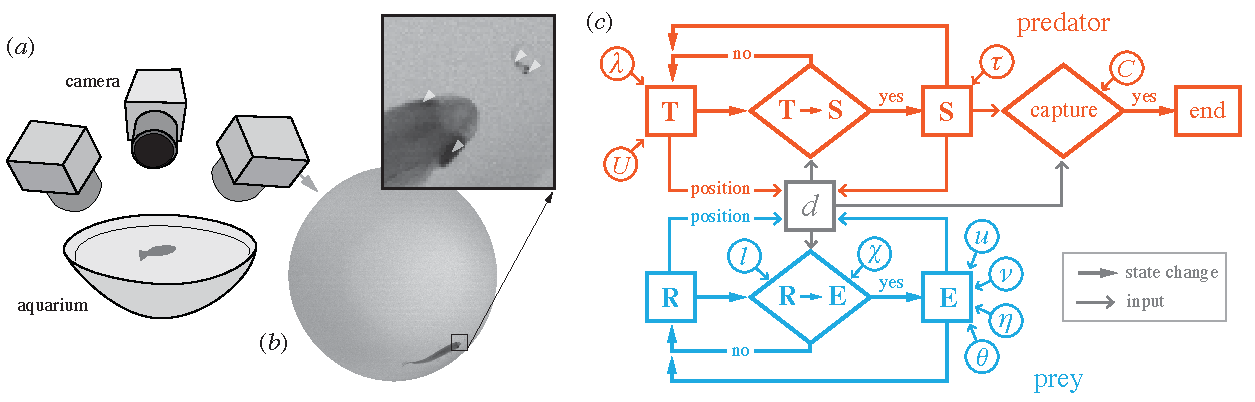
\includegraphics[width=5.5in]{fig1}
\caption{Experimental and mathematical techniques for studying predator-prey interactions. (\textit{a}) Three high-speed video cameras recorded video of one larval prey and one adult predator fish that were placed in a hemispherical aquarium. (\textit{b}) A representative video frame (cropped to the margin of the aquarium) shows an adult in close proximity to the prey. In the inset, white triangles denote the locations of morphological landmarks used to describe the position of the two fish. (\textit{c}) A flow chart illustrates the major components of the game model used to simulate the interactions between predators and prey (see Table \ref{table} for symbol definitions and parameter values).}
\label{fig_setup}
\end{figure}

\pagebreak


\end{document}